\subsection{Conditional Probability and the Multiplication Rule}

\begin{definition}{Conditional Probability}{conditional-probability}
  $E,F$ events, $P(F)>0$:
  \[
    P(E\mid F)=\frac{P(EF)}{P(F)}.
  \]
\end{definition}

\begin{thinking}
  Suppose $F$. Probability of $E$?
  \begin{center}
    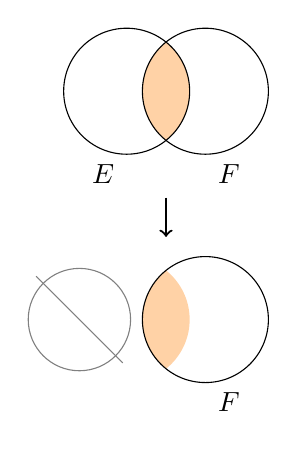
\begin{tikzpicture}
      \begin{scope}
        \clip (1,0) circle (0.8);
        \fill[orange!35] (0,0) circle (0.8);
      \end{scope}
      \draw (0,0) circle (0.8);
      \draw (1,0) circle (0.8);
      \node at (-0.3,-1.05) {$E$};
      \node at (1.3,-1.05) {$F$};
      \draw[->,thick] (0.5,-1.35) -- (0.5,-1.85);
      \draw[gray] (-0.6,-2.9) circle (0.65);
      \draw[gray] (-1.15,-2.35) -- (-0.05,-3.45);
      \begin{scope}
        \clip (1,-2.9) circle (0.8);
        \fill[orange!35] (0,-2.9) circle (0.8);
      \end{scope}
      \draw (1,-2.9) circle (0.8);
      \node at (1.3,-3.95) {$F$};
    \end{tikzpicture}
  \end{center}
\end{thinking}

\[
  \implies P(EF)=P(E\mid F)P(F).
\]

\begin{example}[Two Red Balls]
  $10$ red, $6$ white balls in an urn. Two balls selected from the urn without replacement.
  Probability both red?
  \begin{align*}
    R_1 & =\{\text{first ball is red}\},  \\
    R_2 & =\{\text{second ball is red}\}.
  \end{align*}
  \[
    P(R_1R_2)=P(R_2\mid R_1)P(R_1)
    =\underbrace{\frac9{15}}_{\text{no replacement}}\cdot\frac{10}{16}.
  \]
\end{example}

\begin{theorem}{Multiplication Rule}{multiplication-rule}
  For $\forall E_1,E_2,\ldots,E_n$ events with $P(E_1\cdots E_{n-1})>0$,
  \begin{align*}
    P(E_1E_2\cdots E_n)
     & =P(E_n\mid E_1E_2\cdots E_{n-1})P(E_1\cdots E_{n-1}) \\
     & =P(E_n\mid E_1\cdots E_{n-1})                        \\
     & \quad\cdot P(E_{n-1}\mid E_1\cdots E_{n-2})          \\
     & \quad\cdots                                          \\
     & \quad\cdot P(E_2\mid E_1)                            \\
     & \quad\cdot P(E_1).
  \end{align*}
\end{theorem}

\begin{example}[A Sequence of Red and White Balls]
  There are $6$ white and $5$ red balls in an urn. They are selected without replacement and put in line as drawn.
  \[
    \begin{array}{ccccccccccc}
      R & R & W & W & W & R & W & R & W & W  & R  \\ \hline
      1 & 2 & 3 & 4 & 5 & 6 & 7 & 8 & 9 & 10 & 11
    \end{array}
  \]
  \begin{align*}
    R_i & =\{\text{red ball at }i\text{th draw}\},   \\
    W_i & =\{\text{white ball at }i\text{th draw}\}.
  \end{align*}
  For this sequence,
  \begin{align*}
     & P(R_1R_2W_3W_4W_5R_6W_7R_8W_9W_{10}R_{11})                                  \\
     & \quad=P(R_{11}\mid W_{10}W_9R_8W_7R_6W_5W_4W_3R_2R_1)                       \\
     & \qquad\quad\cdot P(W_{10}\mid W_9R_8W_7R_6W_5W_4W_3R_2R_1)\cdots P(R_1)     \\
     & \quad=\frac11\cdot\frac12\cdot\frac23\cdot\frac24\cdot\frac35
    \cdot\frac36\cdot\frac47\cdot\frac58\cdot\frac69\cdot\frac4{10}\cdot\frac5{11} \\
     & \quad=\frac{5!\,6!}{11!}=\frac1{462}.
  \end{align*}
\end{example}

\begin{example}[Back to the Matching Problem]
  Recall $n$ keys matching $n$ people.
  \[
    E_i=\{\text{person }i\text{ gets it right}\}.
  \]
  Suppose $i_1,i_2,\ldots,i_k$ get their keys right and no one else does.
  \[
    G=\{\text{everyone else gets it wrong}\}.
  \]
  \[
    P(E_{i_1}E_{i_2}\cdots E_{i_k}G)
    =P(G\mid E_{i_1}\cdots E_{i_k})P(E_{i_1}\cdots E_{i_k}).
  \]
  Recall
  \[
    e^x=\sum_{j=0}^{\infty}\frac{x^j}{j!},\qquad
    e^{-1}=\sum_{j=0}^{\infty}\frac{(-1)^j}{j!}.
  \]
  Let
  \[
    p_n=\sum_{j=0}^{n}\frac{(-1)^j}{j!}.
  \]
  \[
    P(\text{no matching of }n\text{ people})=p_n.
  \]
  Let $E=E_{i_1}\cdots E_{i_k}$. Then
  \[
    P(G\mid E)=p_{n-k},\qquad P(EG)=P(G\mid E)P(E).
  \]
  By Theorem~\ref{thm:multiplication-rule},
  \begin{align*}
    P(E) & =P(E_{i_k}\mid E_{i_1}\cdots E_{i_{k-1}})P(E_{i_1}\cdots E_{i_{k-1}}) \\
         & =\cdots,
  \end{align*}
  in which
  \[
    P(E_{i_1})=\frac1n,\qquad P(E_{i_2}\mid E_{i_1})=\frac1{n-1}.
  \]
  Thus
  \[
    P(E)=\frac1n\frac1{n-1}\cdots\frac1{n-k+1}=\frac{(n-k)!}{n!},
  \]
  \[
    P(EG)=P(G\mid E)P(E)=p_{n-k}\frac{(n-k)!}{n!}.
  \]
  \begin{align*}
    P(\text{exactly }k\text{ people get it right})
     & =\sum_{1\le i_1<\cdots<i_k\le n}P(E_{i_1}\cdots E_{i_k}G) \\
     & =\binom nk p_{n-k}\frac{(n-k)!}{n!}                       \\
     & =\frac1{k!}p_{n-k}.
  \end{align*}
\end{example}

\subsection{Conditioning on Cases}

$E,F$ two events:
\[
  E=EF\cup EF^c,\qquad EF\cap EF^c=\varnothing.
\]
\begin{center}
  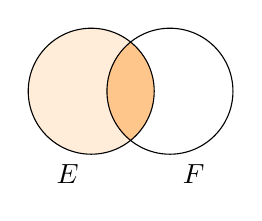
\begin{tikzpicture}
    \fill[orange!15] (0,0) circle (0.8);
    \begin{scope}
      \clip (1,0) circle (0.8);
      \fill[orange!45] (0,0) circle (0.8);
    \end{scope}
    \draw (0,0) circle (0.8);
    \draw (1,0) circle (0.8);
    \node at (-0.3,-1.05) {$E$};
    \node at (1.3,-1.05) {$F$};
  \end{tikzpicture}
\end{center}
For $0<P(F)<1$,
\begin{align*}
  P(E) & =P(EF)+P(EF^c)                      \\
       & =P(E\mid F)P(F)+P(E\mid F^c)P(F^c).
\end{align*}

\begin{example}[Three Cards]
  Three cards: $RR$, $RB$, $BB$. $R$: a red side is showing.
  \begin{align*}
    P(RB\mid R) & =\frac{P(RB\cap R)}{P(R)}       \\
                & =\frac{P(R\mid RB)P(RB)}{P(R)}.
  \end{align*}
  \[
    R=(R\cap RR)\cup(R\cap RB),
  \]
  so
  \[
    P(R)=P(R\mid RR)P(RR)+P(R\mid RB)P(RB).
  \]
  \begin{align*}
    P(RB\mid R)
     & =\frac{P(R\mid RB)P(RB)}{P(R\mid RR)P(RR)+P(R\mid RB)P(RB)}    \\
     & =\frac{\frac12\cdot\frac13}{1\cdot\frac13+\frac12\cdot\frac13}
    =\frac13.
  \end{align*}
\end{example}

\subsection{Total Probability}

Recall Definition~\ref{def:conditional-probability}:
\[
  P(E\mid F)=\frac{P(EF)}{P(F)}.
\]
For $0<P(F)<1$,
\[
  P(E)=P(E\mid F)P(F)+P(E\mid F^c)P(F^c).
\]
Generalized:
\begin{center}
  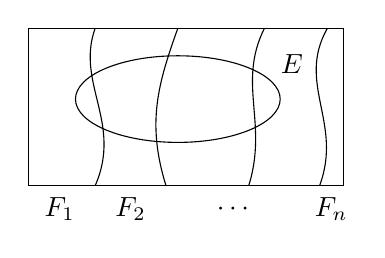
\begin{tikzpicture}
    \draw (0,0) rectangle (4,2);
    \draw (0.85,0) .. controls (1.2,0.8) and (0.6,1.3) .. (0.85,2);
    \draw (1.75,0) .. controls (1.5,0.8) and (1.65,1.3) .. (1.9,2);
    \draw (2.8,0) .. controls (3.05,0.8) and (2.65,1.3) .. (3,2);
    \draw (3.7,0) .. controls (4,0.8) and (3.4,1.3) .. (3.8,2);
    \draw (1.9,1.1) ellipse (1.3 and 0.55);
    \node at (3.35,1.55) {$E$};
    \node at (0.4,-0.3) {$F_1$};
    \node at (1.3,-0.3) {$F_2$};
    \node at (2.6,-0.3) {$\cdots$};
    \node at (3.85,-0.3) {$F_n$};
  \end{tikzpicture}
\end{center}

\begin{theorem}{Law of Total Probability}{total-probability}
  For $F_1,F_2,\ldots,F_n$ disjoint, $\bigcup_{i=1}^n F_i=S$, and $P(F_i)>0$,
  \[
    P(E)=\sum_{i=1}^n P(E\mid F_i)P(F_i).
  \]
\end{theorem}

\begin{example}[Two Types of Coins]
  An urn has type $A,B$ coins. $\frac23$ are $A$, $\frac13$ are $B$.
  \begin{align*}
    P(H\mid A) & =0.6, \\
    P(H\mid B) & =0.4.
  \end{align*}
  \begin{align*}
    P(H) & =P(H\mid A)P(A)+P(H\mid B)P(B)                    \\
         & =\frac23\times0.6+0.4\times\frac13=\frac{1.6}{3}.
  \end{align*}
  \begin{align*}
    P(A\mid H) & =\frac{P(AH)}{P(H)}=\frac{P(H\mid A)P(A)}{P(H)} \\
               & =\frac{0.6\times\frac23}{\frac{1.6}{3}}.
  \end{align*}
\end{example}

\begin{example}[Three Types of Flashlights]
  A bin has three types of flashlights:
  \[
    \begin{array}{c|c|c}
      \text{Type} & \text{Proportion} & P(\text{lasts}>100\text{ hrs}\mid\text{type}) \\ \hline
      1           & 20\%              & 0.7                                           \\
      2           & 30\%              & 0.4                                           \\
      3           & 50\%              & 0.3
    \end{array}
  \]
  Select at random. If it lasts $>100$ hrs, probability of type $1$?
  \begin{align*}
    P(\text{type }1\mid{}>100\text{ hrs})
     & =\frac{P(\text{type }1\cap\{\text{lasts}>100\text{ hrs}\})}{P(>100\text{ hrs})} \\
     & =\frac{P(>100\text{ hrs}\mid\text{type }1)P(\text{type }1)}
    {\displaystyle\sum_{x=1}^3 P(>100\text{ hrs}\mid\text{type }x)P(\text{type }x)}.
  \end{align*}
\end{example}
\begin{example}[Drawing a Die-Determined Number of Balls]
  Suppose an urn has $5$ white, $10$ black balls. A die is rolled; the same number of balls is drawn out. What is the probability all balls are white?
  \[
    E=\{\text{all balls white}\},\qquad
    F_i=\{i\text{ on die}\},\quad i=1,2,3,4,5,6,
    \qquad P(F_i)=\frac16.
  \]
  \begin{align*}
    P(E) & =P(E\mid F_1)P(F_1)+\cdots+P(E\mid F_6)P(F_6)                     \\
         & =\frac16\bigl(P(E\mid F_1)+P(E\mid F_2)+\cdots+P(E\mid F_6)\bigr) \\
         & =\frac16\left(\frac13+\frac{\binom52}{\binom{15}2}
    +\frac{\binom53}{\binom{15}3}+\frac{\binom54}{\binom{15}4}
    +\frac{\binom55}{\binom{15}5}+0\right).
  \end{align*}
\end{example}

\subsection{Independence}

\begin{definition}{Independent Events}{independent-events}
  Events $E,F$ are independent if
  \[
    P(EF)=P(E)P(F).
  \]
  For $P(F)\ne0$, $P(E\mid F)=P(E)$.
\end{definition}

\begin{example}[Rolling a Die Twice]
  Assume we roll a fair die twice.
  \begin{center}
    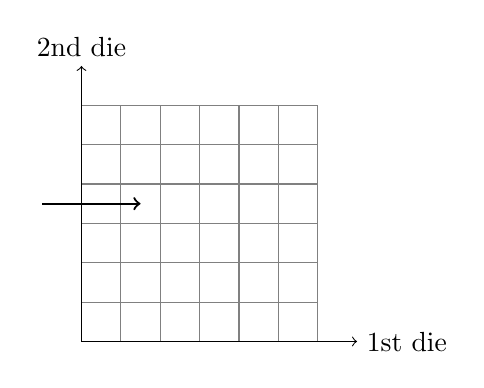
\begin{tikzpicture}[scale=0.5]
      \draw[step=1,gray] (0,0) grid (6,6);
      \draw[->] (0,0) -- (7,0) node[right] {1st die};
      \draw[->] (0,0) -- (0,7) node[above] {2nd die};
      \draw[->,thick] (-1,3.5) -- (1.5,3.5);
    \end{tikzpicture}
  \end{center}
  \begin{align*}
    E_i & =\{\text{1st die rolls }i\}, \\
    F_j & =\{\text{2nd die rolls }j\}.
  \end{align*}
  \[
    P(E_2F_4)=\frac1{36}=P(E_2)P(F_4).
  \]
\end{example}

\subsection{Bernoulli Trials}

\begin{definition}{Bernoulli Trials}{bernoulli-trials}
  An experiment with two outcomes is repeated, and the outcomes on different trials are assumed independent.
  One outcome will be called success and the other failure, and $p$ will be the probability of success on each trial.
\end{definition}

How to define independence for three events $E,F,G$?
\begin{definition}{Independence of Several Events}{mutual-independence}
  For three events $E,F,G$:
  \begin{gather*}
    P(EF)=P(E)P(F),\qquad P(EG)=P(E)P(G),\\
    P(FG)=P(F)P(G),\\
    P(EFG)=P(E)P(F)P(G).
  \end{gather*}
  For $n$ events $E_1,\ldots,E_n$, $\forall\,1\le i_1<\cdots<i_r\le n$,
  $2\le r\le n$,
  \[
    P(E_{i_1}\cdots E_{i_r})=P(E_{i_1})P(E_{i_2})\cdots P(E_{i_r}).
  \]
\end{definition}

For $n$ (independent) Bernoulli trials with outcomes $S$ or $F$ and $P(S)=p$, probability of $k$ successes?
\[
  \begin{array}{cccccc}
    S & S & F & \cdots & S   & F \\ \hline
    1 & 2 & 3 & \cdots & n-1 & n
  \end{array}
\]
One possibility, with $k$ successes:
\[
  P(S_1S_2F_3\cdots S_{n-1}F_n)=P(S)^kP(F)^{n-k}=p^k(1-p)^{n-k}.
\]
All possibilities:
\[
  P(\text{successes}=k)=\binom nk p^k(1-p)^{n-k}.
\]

Probability of 1st success occurring on trial $n$?
\[
  \begin{array}{ccc}
    F & \cdots F & S \\ \hline
    1 & n-1      & n
  \end{array}
  \qquad P(F_1\cdots F_{n-1}S_n)=(1-p)^{n-1}p.
\]

\begin{example}[A Sum of 5 Before 7]
  Two dice are rolled; the sum of the upper faces is recorded. The dice are rolled repeatedly until $5$ or $7$ is shown. Probability of $5$ before $7$?
  \begin{align*}
    E   & =\{5\text{ before }7\},                                \\
    F_1 & =\{5\text{ on 1st roll}\},                             \\
    F_2 & =\{7\text{ on 1st roll}\},                             \\
    F_3 & =\{\text{neither }5\text{ nor }7\text{ on 1st roll}\}.
  \end{align*}
  $F_1,F_2,F_3$ are disjoint and their union is the sample space.
  \[
    P(E)=P(E\mid F_1)P(F_1)+P(E\mid F_2)P(F_2)+P(E\mid F_3)P(F_3).
  \]
  \[
    P(F_1)=\frac4{36},\qquad P(F_2)=\frac6{36},\qquad
    P(F_3)=1-\frac4{36}-\frac6{36}=\frac{26}{36}.
  \]
  \[
    P(E)=1\cdot\frac4{36}+0+
    \underbrace{P(E)}_{\text{1st roll doesn't matter}}\frac{26}{36}.
  \]
  Solve for $P(E)=\dfrac4{10}$.
\end{example}

\subsection{Bayes' Formula}

\begin{theorem}{Bayes' Formula}{bayes-formula}
  For $E_1,\ldots,E_n$ disjoint with union $S$, $P(E_i)>0$, and $P(F)>0$,
  \[
    P(E_j\mid F)=\frac{P(F\mid E_j)P(E_j)}
    {\displaystyle\sum_{i=1}^n P(F\mid E_i)P(E_i)}.
  \]
\end{theorem}
